\newpage
\subsection{Concurrency Control (CC)}
\label{sec:concurrency-control}
The goal of concurrency control is to ensure the correct executions of concurrent transactions.
The baseline for correctness is, as previously mentioned, serial execution.

\inlinedefinition[Serial History] A history $H$ is serial if, for every pair of two transactions $T_i$ and $T_j$ that appear in $H$,
either all operations from $T_i$ appear before all all operations of $T_j$, or vice versa.
A serial history with only committed transactions is correct by definition, because transactions are isolated and each transaction starts in a consistent state
and leaves the DB in a consistent state.

\inlinedefinition[Equivalent History] Two histories are equivalent if and only if
\begin{enumerate}
    \item They are over the same transactions and contain the same operations
    \item Conflicting operations of non-aborted transactions are ordered in the same way in both histories
\end{enumerate}

\inlinedefinition[(Conflict) Serializable History] A history is serializable if and only it is equivalent to a serial history.

A history is guaranteed to \textit{not} be CS if there are conflicting operations as defined on the previous page.

\inlinetheorem[Serializability] A history is serializable if and only if its serializability graph is acyclic.
The serializabililty graph is constructed from the history graph as follows:
\begin{enumerate}
    \item The start node is the transaction the first operation.
    \item Then, follow the operations, adding any new transaction to the tree and connect any further dependencies.
\end{enumerate}
More visually, see the below graphics

\begin{figure}[h!]
    \begin{center}
        \begin{subfigure}{0.49\textwidth}
            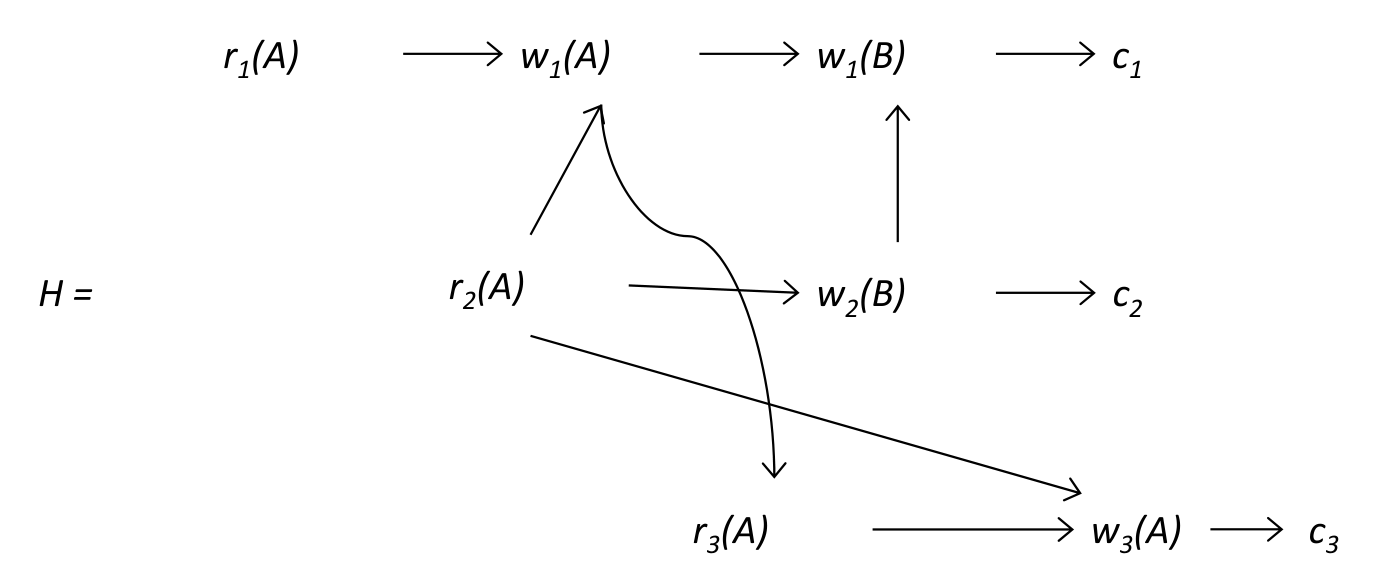
\includegraphics[width=0.9\textwidth]{assets/serializability-graph-history.png}
            \caption{The history}
        \end{subfigure}
        \begin{subfigure}{0.49\textwidth}
            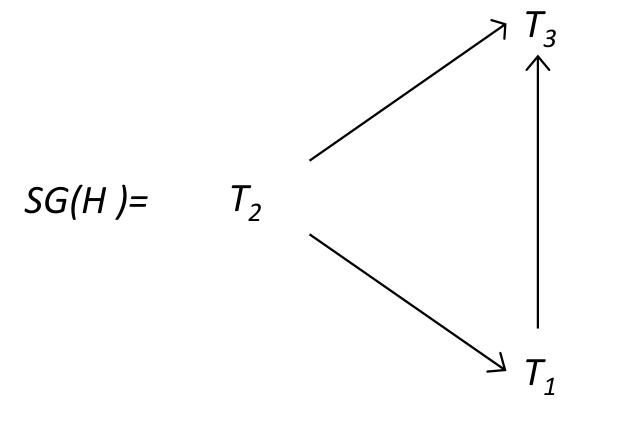
\includegraphics[width=0.7\textwidth]{assets/serializability-graph-built.png}
            \caption{The resulting serializability graph}
        \end{subfigure}
    \end{center}
    \caption{Building a serializability graph (Figure from lecture slides 19, slide 37 and 38)}
\end{figure}

\subsubsection{Building a serializability graph}
Since the above guide may not be very easy to understand, a more intuitive approach\footnote{Adapted from \url{https://www.siemens.blog/posts/serializability-theory/}}:
\begin{enumerate}
    \item Write down in rows the operations of each thread, such that on the horizontal axis they still align in the way they did when written down in a line
    \item Add edges horizontally (as the operations of each thread depend on each other implicitly)
    \item Add edges between successive write operations to the same field
    \item Add edges between writes and successive reads of the same field (for all threads, doesn't have to be the next operation)
    \item Add edges between reads and successive writes that happen before the reading thread commits
\end{enumerate}
Then, from this history graph notation, derive the serializability graph by only considering the edges between the threads.
The serialization order is then determined by the topological ordering and the graph is not serializable if there exists a cycle
(as there doesn't exist a topological ordering)
